\Problem{Дома в Colorville}{1}{64}{buildings.in}{buildings.out}

\Legend
Как путешествующий продавец в глобализированном мире, Алан всегда много двигался. Он почти никогда
не жил в одном и том же городе больше нескольких лет, пока его сердце не тосковало по другому месту.
Тем не менее, этот новейший город все еще его любимый - он такой красочный. Алан недавно переехал
в Colorville, маленький город между некоторыми действительно хорошими горами. Здесь Алан наконец-то
решил поселиться и построить себе дом - хороший большой дом, чтобы назвать его собственным.
В Colorville, у многих людей есть свои собственные дома - каждый окрашен различным шаблоном цветов
так, что никакие два дома не выглядят одинаково. Каждая стена состоит из ровно $n \cdot n$ квадратов,
каждый из которых окрашен в определенный цвет (окна и двери также рассматриваются как уникальные
``цвета''). Стены дома расположены в форме правильного $m$-угольника, с крышей сверху. Согласно
глубоким традициям Colorville крыши должны показать единство среди жителей Colorville, поэтому все
крыши в Colorville имеют один и тот же цвет.

\begin{center}
	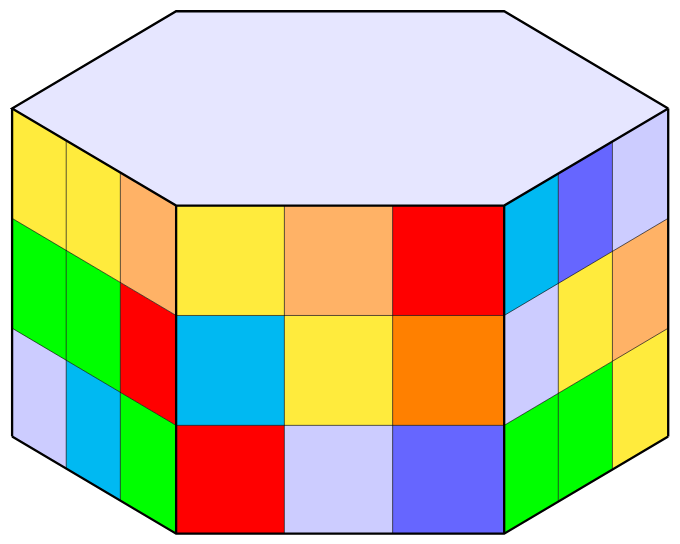
\includegraphics[width=200pt,natwidth=680,natheight=544]{tasks/buildings/statements/images/building.png}
\end{center}

Конечно, Алан хочет следовать этому обычаю, чтобы убедиться, что он вписывается. Однако, есть
так много возможных конструкций на выбор. Можете ли вы сказать Алану, сколько возможных дизайнов
домов существует? (Два проекта дома, очевидно, одинаковы, если они могут быть сведены друг к другу
простым поворотом).

\Input
В единственной строке входных данных содержится три целых числа $n$, $m$ и $c$ ($1 \le n, c \le 500$,
$3 \le m \le 500$)~--- длинна стороны каждой стены (высота так же равна $n$), количество углов у
правильного многоугольника и количество различных цветов соответственно.

\Output
Выведите число $s$~--- количество различных дизайнов домов. Так как $s$ может быть слишком большим,
выведите его по модулю $10^9 + 7$.

\Samples
\BeginTests
\Test{tasks/buildings/tests/samples}{01}{01.a}
\Test{tasks/buildings/tests/samples}{02}{02.a}
\EndTests

\Scoring
\begin{itemize}
	\item $n = 1$, $m \le 4$~--- 20 баллов.
	\item $n = 1$~--- 20 баллов
	\item $m \le 4$~--- 20 баллов.
	\item без ограничений~--- 40 баллов.
\end{itemize}

\EndProblem
